\documentclass[t]{beamer}
\usefonttheme{serif}

\usepackage{amsmath,amsthm,amssymb,amsfonts,amscd,mathrsfs,amsxtra,multirow,kotex,mathtools,gensymb,textcomp,lipsum,tikz,verbatim,color,soul,courier,mdframed,xcolor}
\usepackage[normalem]{ulem}
\usetikzlibrary{calc,matrix,arrows,chains,positioning,scopes}
\usepackage{pdfpages,cancel}

\theoremstyle{plain}
\newtheorem{thm}{Theorem}[section]
\newtheorem{prop}[thm]{Proposition}

\theoremstyle{definition}
\newtheorem{defn}[thm]{Definition}
\newtheorem{exmp}[thm]{Example}
\newtheorem{excs}[thm]{Exercise}
\newtheorem{rem}[thm]{Remark}
\newtheorem{prob}[thm]{Problem}
\newtheorem{cor}[thm]{Corollary}

\newcommand \tr[1]{\textcolor{red}{#1}}
\newcommand{\tikzmark}[1]{\tikz[overlay,remember picture] \node (#1) {};}
\newcommand{\varep}{\varepsilon}
\newcommand{\DrawBox}[1][]{%
    \tikz[overlay,remember picture]{
    \draw[red,#1]
      ($(left)+(-0.2em,0.9em)$) rectangle
      ($(right)+(0.2em,-0.3em)$);}
}

\newcommand{\tikzmarkk}[2]{
    \tikz[overlay,remember picture,baseline] 
    \node[anchor=base] (#1) {$#2$};
}
\newcommand*\circled[1]{\tikz[baseline=(char.base)]{
            \node[shape=circle,draw,inner sep=2pt] (char) {#1};}}

\tikzset{join/.code=\tikzset{after node path={%
\ifx\tikzchainprevious\pgfutil@empty\else(\tikzchainprevious)%
edge[every join]#1(\tikzchaincurrent)\fi}}}

\tikzset{>=stealth',every on chain/.append style={join},
         every join/.style={->}}
\tikzstyle{labeled}=[execute at begin node=$\scriptstyle,
   execute at end node=$]

\newenvironment<>{proofs}[1][\proofname]{%
   \par
   \def\insertproofname{#1\@{.}}%
   \usebeamertemplate{proof begin}#2}
 {\usebeamertemplate{proof end}}
 

\addtobeamertemplate{navigation symbols}{}{%
    \usebeamerfont{footline}%
    \usebeamercolor[fg]{footline}%
    \hspace{1em}%
    \raisebox{2pt}[0pt][0pt]{\insertframenumber/\inserttotalframenumber}
}
\setbeamercolor{footline}{fg=blue}
\setbeamerfont{footline}{series=\bfseries}
\title[]{SE102:Multivariable Calculus}

\author[]{Hyosang Kang\inst{1}}

\institute[]{\inst{1}Division of Mathematics\\ School of Interdisciplinary Studies\\ DGIST}

\date[]{Week 11}

\begin{document}

\begin{frame}
\titlepage
\end{frame}

\begin{frame}
\begin{defn}
Let $\varphi(x,y)$ be a function defined on a region $D\subset\mathbf R^2$.
The vector field $\nabla\varphi$ is called the \textbf{gradient vector field} of $\varphi$.
Conversely, let $\mathbf F:D\to\mathbf R^2$ be a vector field defined on $D$.
A function $\varphi(x,y)$ satisfying
	\[\nabla\varphi = (\varphi_x,\varphi_y) =\mathbf F\]
is called the \textbf{potential function} of $\mathbf F$.
\end{defn}
\end{frame}

\begin{frame}
\begin{defn}
Let $\mathbf F(x,y)=(P(x,y),Q(x,y))$. 
If $Q_x-P_y=0$, then $\mathbf F$ is called a \textbf{closed} vector field.
\end{defn}
\begin{thm}
If a vector field $\mathbf F$ admits a potential function, 
then it is closed.
\end{thm}
\begin{proof}
Suppose that $\mathbf F = (P,Q) = \nabla \varphi$. Then
	\[Q_x-P_y = \varphi_{yx}-\varphi_{xy} = 0.\]
\end{proof}
\end{frame}

\begin{frame}
\begin{defn}
A vector field $\mathbf F$ defined on $D\subset\mathbf R^2$
is called \textbf{conservative} if the line integral 
$\displaystyle\int_C\mathbf F\cdot d\mathbf s$
only depends on the start and end point of the curve $C\subset D$.
In other words, the vector field is conservative 
if \[\oint_C\mathbf F\cdot d\mathbf s=0\] 
for any closed curve $C\subset D$.
\end{defn}
\end{frame}

\begin{frame}
\begin{thm}
If a vector field $\mathbf F$ admits a potential function, 
then it is conservative.
\end{thm}
\begin{proof}
Let $c(t) = (x(t),y(t))$, $a\le t\le b$ be a parametrization of $C$ from $p_0=c(a)$ to $p_1=c(b)$.
Note that
	\[\int_C \mathbf F \cdot d\mathbf s = \int_C \varphi_xdx + \varphi_ydy = \int_a^b \frac{\partial\varphi}{\partial x} \frac{\partial x}{\partial t} + \frac{\partial\varphi}{\partial y}\frac{\partial y}{\partial t} dt \]
By the Chain rule, we getn
	\[ \int_a^b \frac{\partial\varphi}{\partial x} \frac{\partial x}{\partial t} + \frac{\partial\varphi}{\partial y}\frac{\partial y}{\partial t} dt = \int_a^b \frac{d}{dt} \varphi(x(t),y(t))dt = \varphi(p_1)-\varphi(p_0).\]
\end{proof}
\end{frame}

\begin{frame}
\begin{cor}
If a vector field $\mathbf F$ admits a potential function on $D$, 
then
	\[\oint_C\mathbf F\cdot d\mathbf s=0\]
for any closed curve $C$ in $D$. 
\end{cor}
\begin{exmp}
Let $D=\{(x,y)\,|\,x,y>0\}$ be the first quadrant on $\mathbf R^2$. The function
	\[\theta(x,y)=\tan^{-1}\left(\frac{y}{x}\right)\]
is a potential function of the vector field 
$$\mathbf A = \displaystyle 
	\left(-\frac{y}{x^2+y^2},\frac{x}{x^2+y^2}\right)$$
on $D$.
\end{exmp}
\end{frame}

\begin{frame}
\begin{exmp}
Not every closed vector field admits a potential function.
Consider the vector field 
$$\mathbf A = \displaystyle 
	\left(-\frac{y}{x^2+y^2},\frac{x}{x^2+y^2}\right)$$
defined on $D = \mathbf R^2\setminus\{(0,0)\}$.
is closed, but it does not admit any potential function on $D$.
(Think carefully why this does not contradict to the previous example.)
To show this, suppose that $\mathbf a$ has a potential function 
on $\mathbf R^2\setminus\{(0,0)\}$.
Then $\displaystyle \oint_C\mathbf a\cdot d\mathbf s$ must be $0$ 
for any closed curve $C$.
However we can show that the line integral of this vector field 
over a circle around the origin is not zero.
\end{exmp}
\end{frame}

\begin{frame}
\begin{thm}[Green]
Let $D$ be a connected region in $\mathbf R^2$
bounded by piecewise differentiable curve $C$.
Let $\mathbf F(x,y)=(P(x,y), Q(x,y))$ be a vector field defined on $D$.
Then 
	\[\oint_C\mathbf F\cdot d\mathbf s=\iint_D Q_x-P_y dA\]
where the curve $C$ is \underline{positively oriented}.
\end{thm}
\end{frame}

\begin{frame}
\begin{proof}
Suppose that the region $D$ is given by
	\[D = \{(x,y) \,|\, a\le x\le b, g_1(x)\le y\le g_2(x)\}\]
Then
	\begin{align*}
	\oint_C Pdx 
	&= \int_a^b P(x,g_1(x))dx + \int_b^a P(x,g_2(x))dx \\
	&= \int_a^b P(x,g_1(x))-P(x,g_2(x)) dx = - \iint_D P_y dA
	\end{align*}
Similarly, $\displaystyle \int_CQdy = \iint_D Q_x dA$.
\end{proof}
\end{frame}


\begin{frame}
\begin{cor}
Let $D$ be a \underline{simply connected} region in $\mathbf R^2$.
A vector field $\mathbf F$ defined on $D$ is conservative if it is closed.
\end{cor}
\begin{thm}[Poincare lemma]
Let $D$ be a \underline{simply connected} region in $\mathbf R^2$ 
and $\mathbf F$ a vector field defined on $D$.
If $\mathbf F$ is closed, then $\mathbf F$ admits a potential function.
Furthermore, if $D$ is connected, 
then the potential function is unique up to constant.
\end{thm}
\end{frame}

\begin{frame}
\begin{proof}
Let $p_0$ be a point in $D$. For $p=(x,y)$ in $D$, let us define a function $\varphi(x,y)$ as follows.
	\[\varphi(x,y) = \int_{p_0}^p\mathbf F\cdot d\mathbf s=\int_{p_0}^pPdx+Qdy\]
The function $\varphi(x,y)$ is well-defined.
Suppose that the path in the integral near $p$ is given by $c(t) = (x+t,y)$, $\epsilon\in(-\epsilon,0]$. 
Then
	\[\varphi_x = \frac{\partial}{\partial x}\int_{(x-\Delta x,y)}^{(x,y)} Pdx = P.\]
We can show $\varphi_y = Q$ in a similar way.
\end{proof}
\end{frame}

\begin{frame}
\begin{exmp}
Let $C$ be the semicircular arc from $(0,2)$ to $(0,-2)$ oriented counter-clockwise.
Evaluate
\[\int_Cxy^2dx-xydy\]
\end{exmp}
\begin{exmp}
Let $C$ be the circle $(x-2)^2+(y-3)^2=1$ oriented counter-clockwise. Evaluate
\[\int_C\left(y-\log(x^2+y^2)\right) dx + \left(2\tan^{-1}(y/x)\right) dy\]
\end{exmp}
\end{frame}

\begin{frame}
\begin{exmp}
Let $(a_1,b_1)$, $(a_2,b_2)$, $\cdots$, $(a_n,b_n)$ be the successive vertices
of $n$-polygon. Show that the area inside the polygon is
	$$\frac{1}{2}\left(\left|\begin{matrix}a_1 & b_1\\a_2 &b_2\end{matrix}\right|+
	\left|\begin{matrix}a_2 & b_2\\a_3 &b_3\end{matrix}\right|+ \cdots +
	\left|\begin{matrix}a_{n-1} & b_{n-1}\\a_n &b_n\end{matrix}\right| +
	\left|\begin{matrix}a_n & b_n\\a_1 &b_1\end{matrix}\right|\right)$$
\end{exmp}
\end{frame}

\begin{frame}
\begin{prob}
Let $\mathbf F = \langle 3y,-4x\rangle$.
Find $\displaystyle\oint_{\partial D} \mathbf F\cdot d\mathbf s$
oriented counter-clockwise for the following region $D$.
	\begin{enumerate}
		\item $\displaystyle D= \{(x,y)\,|\,x^2+y^2\le 4\}$
		\item $\displaystyle D = \{(x,y,)\,|\,x^2+2y^2\le 4\}$
	\end{enumerate}
\end{prob}
\end{frame}

\begin{frame}
\begin{prob}
Evaluate $\displaystyle\oint_C 5ydx-3xdy$ where $C$ is the cardioid $r=1-\sin\theta$
oriented counter-clockwise.
\end{prob}
\end{frame}

\begin{frame}
\begin{prob}
Evaluate $\displaystyle\oint_C (x^4y^5-2y)dx + (3x+x^5y^4)dy$ where
$C$ is as shown below.
\begin{center}
	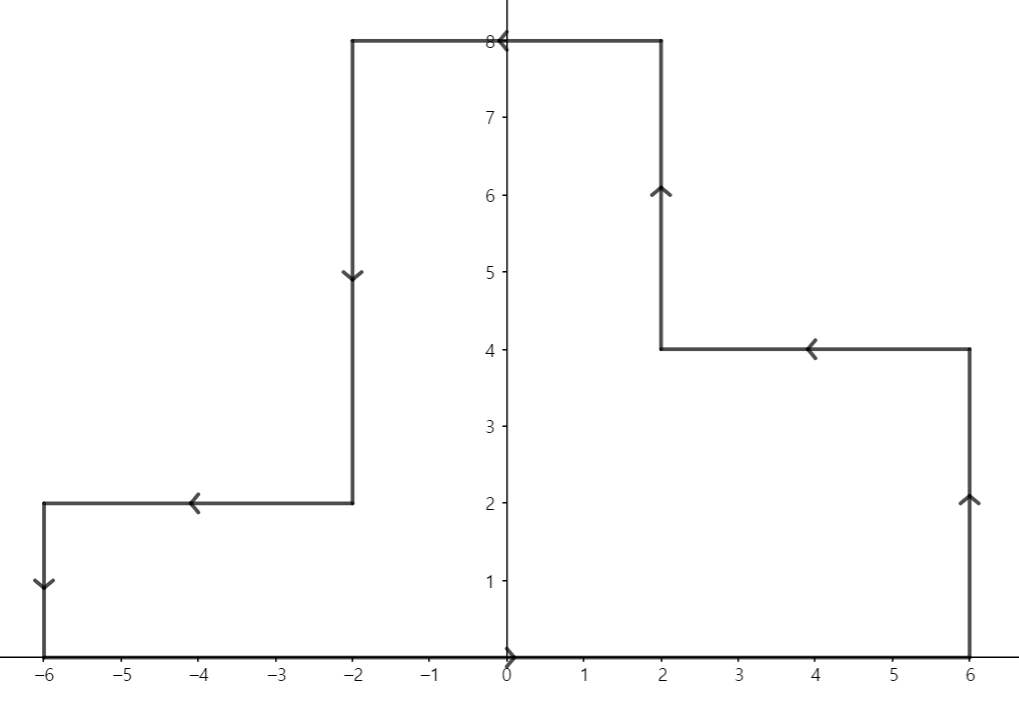
\includegraphics[scale=.5]{image/lnsec11-1}
\end{center}
\end{prob}
\end{frame}

\begin{frame}
\begin{prob}
Determine the value of
\[\oint_C\frac{xdx+ydy}{x^2+y^2}\]
where $C$ is a simple closed curve enclosing the origin
oriented counter-clockwise.
\end{prob}	
\end{frame}

\end{document}
